\documentclass[a4paper,12pt,twocolumn]{article}

\usepackage{times}
\usepackage[utf8]{inputenc}
\usepackage[brazil]{babel}
\usepackage[a4paper,margin=2cm,columnsep=1cm]{geometry}
\usepackage{authblk}
\usepackage{titlesec}
\usepackage[pdftex]{graphicx}
\usepackage{mathtools}
\usepackage{amsmath}
\usepackage{enumitem}
\usepackage[font={small}]{caption}

\topmargin      0.0cm
\headheight     0.0cm
\headsep        0.0cm
\oddsidemargin  0.0cm
\evensidemargin 0.0cm
\textheight     22.86cm
\textwidth      16.51cm

\graphicspath{{images/}}
\titleformat*{\section}{\normalsize\bfseries\filcenter}
\titleformat*{\subsection}{\normalsize\bfseries\filcenter}

\renewcommand{\figurename}{\small Figure}
\newcommand{\figureref}[1]{Fig. (\ref{fig:#1})}
\newcommand{\equationref}[1]{Eq. (\ref{eq:#1})}
\newcommand{\bigsum}{\displaystyle\sum}
\newcommand{\twopartdef}[4]
{
    \left\{
        \begin{array}{ll}
            #1 & \mbox{se } #2 \\
            #3 & \mbox{se } #4
        \end{array}
    \right.
}


\begin{document}

\title{\textbf{Resumo de Aprendizagem de Máquina 2014-2}}
\author{
    \textbf{Eduardo M. B. de A. Tenório}\\
    \small{\texttt{embat@cin.ufpe.br}}
}
\affil{\large CIn-UFPE}
\date{}

\maketitle


\begin{abstract}
\begin{itshape}
Este documento tem por finalidade ser um resumo dos assuntos abordados na disciplina \emph{Aprendizagem de Máquina} do período 2014-2 do CIn-UFPE, ministrada pelos professores Francisco Carvalho e Teresa Ludermir. A maioria do documento referencia o livro ``Pattern Classification", de Duda, Hart \& Stork. Os códigos utilizados como exercício de fixação encontram-se em \normalfont{github.com/embatbr/resumo-aprendizagem}.
\end{itshape}
\end{abstract}


\section{Teoria da Decisão Bayesiana}

\subsection{Introdução}

Teoria da Decisão Bayesiana é uma abordagem estatística para a classificação de
padrões, baseada em quantificar os tradeoffs associados a tomar uma determinada
decisão (classificar) utilizando probabilidade e considerando os custos associados.

O \textbf{estado natural} é denotado por $\omega$, de modo que $\omega = \omega_i$, para $i = 1, 2, ..., c$, significa que o exemplo foi classificado como pertencente à classe $\omega_i$. Cada uma dessas classes possui uma \textbf{probabilidade a priori} $P(\omega_i)$, com

\begin{equation}
    \sum_{i=1}^{c} P(\omega_i) = 1,
    \label{eq:sum_priori_prob_to_one}
\end{equation}

\noindent refletindo o conhecimento prévio da chance de um elemento da classe $\omega_i$ aparecer. A \textbf{regra de decisão} fica:

\begin{equation}
    \text{Decida } \omega_i \text{ se } i = \max_j P(\omega_j).
    \label{eq:decision_1}
\end{equation}

\noindent Neste caso a classe $\omega_i$ sempre é escolhida e a probabilidade de erro é dada por:

\begin{equation}
    P_{err}(\omega_i) = 1 - P(\omega_i).
    \label{eq:prob_i_error}
\end{equation}

Utilizando uma característica $x$ que seja contínua e aleatória, sua \textbf{densidade de probabilidade estado-condicional} é dada por $p(x|\omega)$. Logo, a diferença entre $p(x|\omega_i)$ e $p(x|\omega_j)$ descreve a diferença da característica $x$ entre as populações das classes $\omega_i$ e $\omega_j$.

\begin{figure}[ht]
    \centering
    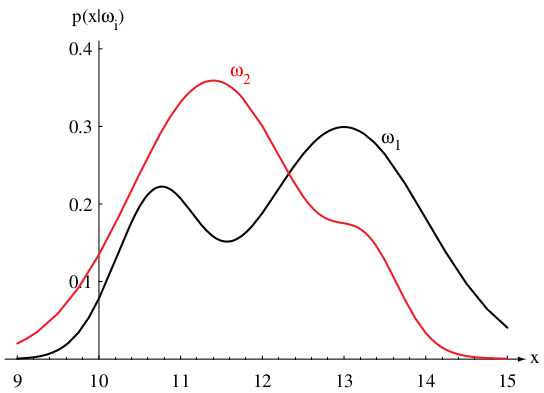
\includegraphics[scale=0.4]{state-conditional_pdf}
    \caption{Para $\omega_i = \omega_2$, é mais frequente observar $x$ entre 11 e 12 que $x = 13$ (valor mais provável se $\omega_i = \omega_1$).}
    \label{fig:state-conditional_pdf}
\end{figure}

Sabendo $P(\omega_i)$ e $p(x|\omega_i)$, e medindo um valor $x$, a probabilidade conjunta de achar um padrão na classe $\omega_i$ e com $x$ é dado por: $p(\omega_i,x) = P(\omega_i|x)p(x) = p(x|\omega_i)P(\omega_i)$, que pela \textbf{fórmula de Bayes} fica:

\begin{equation}
    P(\omega_i|x) = \frac{p(x|\omega_i)P(\omega_i)}{p(x)},
    \label{eq:bayes}
\end{equation}

\noindent com a evidência para $c$ classes
\begin{equation}
    p(x) = \sum_{j=1}^c p(x|\omega_j)P(\omega_j).
    \label{eq:bayes}
\end{equation}

A probabilidade a posteriori das classes $\omega_1$ e $\omega_2$ para um conjunto de valores de $x$ é mostrada em \figureref{posteriori_prob}. A regra de decisão fica:
\begin{equation}
    \text{Decida } \omega_i \text{ se } \omega_i \text{ minimiza } P(erro|x),
    \label{eq:decision_2}
\end{equation}

\noindent onde

\begin{equation}
    P(erro|x) = \sum_{j\neq i} P(\omega_j|x),
    \label{eq:bayes}
\end{equation}

\noindent ou simplesmente $P(erro|x) = 1 - P(\omega_i|x)$. Então a regra torna-se:

\begin{equation}
    \text{Decida } \omega_i \text{ se } i = \max_j P(\omega_j|x),
    \label{eq:decision_3}
\end{equation}

\begin{figure}[ht]
    \centering
    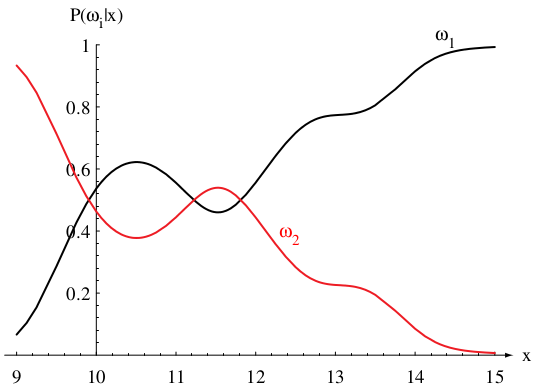
\includegraphics[scale=0.4]{posteriori_prob}
    \caption{Probabilidades a posteriori para $P(\omega_1) = \frac{2}{3}$ e $P(\omega_2) = \frac{1}{3}$, e para as densidades de probabilidade estado-condicional mostradas em \figureref{state-conditional_pdf}.}
    \label{fig:posteriori_prob}
\end{figure}

Esta regra minimiza a probabilidade média de erro, dada por

\begin{equation}
    P(erro) = \int_{-\infty}^{\infty} P(erro|x)p(x) dx.
    \label{eq:bayes}
\end{equation}

\subsection{Características Contínuas}

É de fácil compreensão que a característica $x$ pode ser trocada por um vetor de características $\mathbf{x} = (x_1, x_2, ..., x_d)$, onde $\mathbf{x}$ pertence ao espaço $\mathbf{R}^d$ (espaço de características). A região que decide $\omega_i$ é denotada por $\mathcal{R}_i$.

Outras ações além de apenas classificar um elemento podem ser tomadas, como por exemplo a \textbf{rejeição}: recusar-se a tomar uma decisão; uma opção válida quando o custo de ser indeciso é aceitável. Para isso \textbf{funções de custo} são inseridas, permitindo tratar de situações onde alguns erros de classificação são mais importantes que outros.

Seja $\{\omega_1, ..., \omega_c\}$ o conjunto finito de $c$ classes e seja $\{\alpha_1, ..., \alpha_a\}$ o conjunto finito de possíveis ações. A função de custo $\lambda(\alpha_i|\omega_j)$ descreve o custo de tomar a ação $\alpha_i$ quando a classe é $\omega_j$. Logo, observado um $\mathbf{x}$ em particular, tomar a ação $\alpha_i$ quando a classe é $\omega_j$ leva a um custo esperado (\textbf{risco})

\begin{equation}
    R(\alpha_i|\mathbf{x}) = \sum_{j=1}^c \lambda(\alpha_i|\omega_j) P(\omega_j|\mathbf{x}).
    \label{eq:conditional_risk}
\end{equation}

$R(\alpha_i|\mathbf{x})$ é chamado de \textbf{risco condicional}. Qualquer que seja o $\mathbf{x}$ observado, o risco pode ser minimizado selecionando a ação que minimiza $R(\alpha_i|\mathbf{x})$.

A regra de decisão geral é uma função $\alpha(\mathbf{x})$ que diz qual ação tomar para cada possível observação, ou seja, para cada $\mathbf{x}$ a \textbf{função de decisão} $\alpha(\mathbf{x})$ assume um dos $a$ valores $\alpha_1, ..., \alpha_a$. Logo, o \textbf{risco global} é dado por

\begin{equation}
    R = \int R(\alpha(\mathbf{x}))p(\mathbf{x})d\mathbf{x}.
    \label{eq:conditional_risk}
\end{equation}

O risco global mínimo é chamado de \textbf{risco de Bayes}, denotado por $R^*$, sendo a melhor perfomance alcançável.

\subsection{Classificação por Taxa de Erro Mínima}

Para evitar erros, a regra de decisão procurada é aquela que minimiza a probabilidade de erro, i.e. minimiza a \textbf{taxa de erro}. A função de custo de interesse para este caso é chamada de \textbf{simétrica} ou \textbf{zero-um},

\begin{equation}
    \lambda(\alpha_i|\omega_j) = \twopartdef{0}{i=j}{1}{i \neq j} \hfill i, j = 1, ..., c.
    \label{eq:loss_zero_one}
\end{equation}

Como todos os erros tem custo igual, o risco condicional é dado por

\begin{equation}
    R(\alpha_i|\mathbf{x}) = 1 - P(\omega_i|\mathbf{x})
    \label{eq:conditional_risk_zero_one}
\end{equation}

\noindent com $P(\omega_i|\mathbf{x})$ sendo a probabilidade condicional da ação $\alpha_i$ estar correta. A regra de decisao neste caso continua:
\begin{equation}
    \text{Decida } \omega_i \text{ se } i = \max_j P(\omega_j|x).
    \label{eq:decision_4}
\end{equation}

\begin{figure}[ht]
    \centering
    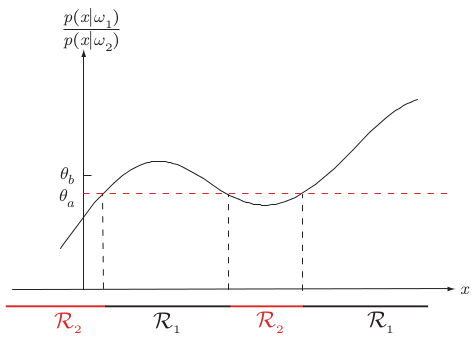
\includegraphics[scale=0.5]{decision_region}
    \caption{Se a penalização de classificar $\omega_1$ como $\omega_2$ for maior que o oposto, então a razão tende ao threshold $\theta_b$.}
    \label{fig:decision_region}
\end{figure}

\subsection{Funções Discriminantes}

A maneira mais usual de representar classificadores de padrões é através de um conjunto de \textbf{funções discriminantes} $g_i(\mathbf{x}), i = 1, ..., c$. O classificador atribui um vetor de características $\mathbf{x}$ à classe $\omega_i$ se

\begin{equation}
    g_i(\mathbf{x}) = \max_j g_j(\mathbf{x})
    \label{eq:discriminant_functions}
\end{equation}

\begin{figure}[ht]
    \centering
    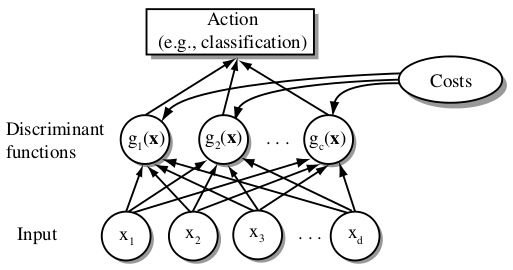
\includegraphics[scale=0.45]{discriminant_functions}
    \caption{Classificador com $c$ funções discriminantes e entradas $d$-dimensional. A ação geralmente é ``escolher o maior $g_i(\mathbf{x})$".}
    \label{fig:discriminant_functions}
\end{figure}

Para o caso geral com riscos, pode-se fazer $g_i(\mathbf{x}) = - R(\alpha_i|\mathbf{x})$, enquanto para o caso ``taxa de erro mínima", $g_i(\mathbf{x}) = P(\omega_i|\mathbf{x})$. A função discriminante $g_i(\mathbf{x})$ pode ser substituída por $f(g_i(\mathbf{x}))$, com $f(\cdot)$ sendo uma função monotonicamente crescente (e.g. logaritmo), com o resultado da classificação ficando inalterado. Como resultado, $\mathbf{R}^d$ é dividido em regiões de decisão $\mathcal{R}_i$ (não necessariamente conectadas) para cada classe $\omega_i$.

Para o caso em que $c = 2$, o classificador é chamado \textbf{dicotomizador}, e apenas uma função discriminante $g(\mathbf{x}) \equiv g_1(\mathbf{x}) - g_2(\mathbf{x})$ é necessária. Logo a regra de decisão torna-se:
\begin{equation}
    \text{Decida } \omega_1 \text{ se } g(\mathbf{x}) > 0 \text {; senão, } \omega_2.
    \label{eq:decision_4}
\end{equation}

\subsection{Características Discretas}

Em muitas aplicações práticas as componentes de $\mathbf{x}$ são valores inteiros binários, ternários ou outro de ordem mais alta, de modo que $\mathbf{x}$ pode assumir apenas um dos $m$ valores discretos $\mathbf{v_1}, ..., \mathbf{v_m}$. Nestes casos, a função de densidade de probabilidade $p(\mathbf{x}|\omega_j)$ torna-se uma função de massa de probabilidade $P(\mathbf{x}|\omega_j)$ e

\begin{equation}
    \int p(\mathbf{x}|\omega_j) d\mathbf{x}
    \label{eq:integral_pdf}
\end{equation}

\noindent é substituída por

\begin{equation}
    \sum_\mathbf{x} P(\mathbf{x}|\omega_j).
    \label{eq:sum_pmf}
\end{equation}

\noindent Na fórmula de Bayes as densidades de probabilidade são trocadas por probabilidades

\begin{equation}
    P(\omega_j|\mathbf{x}) = \frac{P(\mathbf{x}|\omega_j)P(\omega_j)}{P(\mathbf{x})}
    \label{eq:bayes_discrete}
\end{equation}

onde

\begin{equation}
    P(\mathbf{x}) = \sum_{j=1}^c P(\mathbf{x}|\omega_j)P(\omega_j).
    \label{eq:bayes_discrete}
\end{equation}

A definição do risco condicional $R(\alpha|\mathbf{x})$ mantém-se inalterada.

\section{Estimação Paramétrica}

TODO ler seções 3.1, 3.2, 3.8 do Duda, Hart \& Stork

\end{document}